\section{Evaluation}
\label{sec:evaluation}

We evaluate \sysname{} for its flexibility and performance.

\begin{itemize}[leftmargin=30pt]
\item[\autoref{sec:expressivity}] Does \sysname{} provide sufficiently expressive
  APIs that can be used in applications?
\item[\autoref{sec:degr-perf}] How effective is \sysname{}'s degradation scheme
  work in comparison to applications developed without the degradation?
\item[\autoref{sec:overhead}] What's the overhead of using \sysname{}?
\end{itemize}

Our evaluation shows that the APIs provided by \sysname{} is sufficiently
flexible that non-trivial real-world applications can be built atop. In
comparison to alternative behaivor (such as \texttt{RandomDrop},
\texttt{BurstDrop} and \texttt{Backlogged}), our degradation scheme offers a
significantly small accuracy drop (10\% instead of 80\%).

\subsection{Building Streaming Applications}
\label{sec:expressivity}

In this section, we describe our experience of using \sysname{} to build two
real-world applications: one in video processing domain; one in log-analysis
domain. They align well with our motivating applications mentioned in \autoref{sec:motiv-appl}.

\begin{figure}
  \begin{lstlisting}
WaspManager::new(test_source, prod_source, scoring, |source| {
    source.skip_unless(|&i| i < 3)
        .maybe_downsample(2)
        .tumbling_window(2, |v: Vec<usize>| v.iter().sum::<usize>())
        .compose()
}).run()
  \end{lstlisting}
  \caption{Snippet of CDN analytics application code doing windowed sum.}
  \label{fig:cdn-code}
\end{figure}

\subsection{Degradation Performance}
\label{sec:degr-perf}

In this section we evaluate how the application behaves when the available
resource (bandwidth in this context) is not sufficient. Specifically, we compare
the generated degradation scheme (called \texttt{ApplicationAware}) with
alternative schemes such as \texttt{RandomDrop}, \texttt{BurstDrop}, and
\texttt{Backlogged}. The drop behavior is similar to what one would expect in
UDP-like transport protocol while the backlogged one is a common choice for
stream processing frameworks that uses TCP.

\begin{figure}
  \centering
  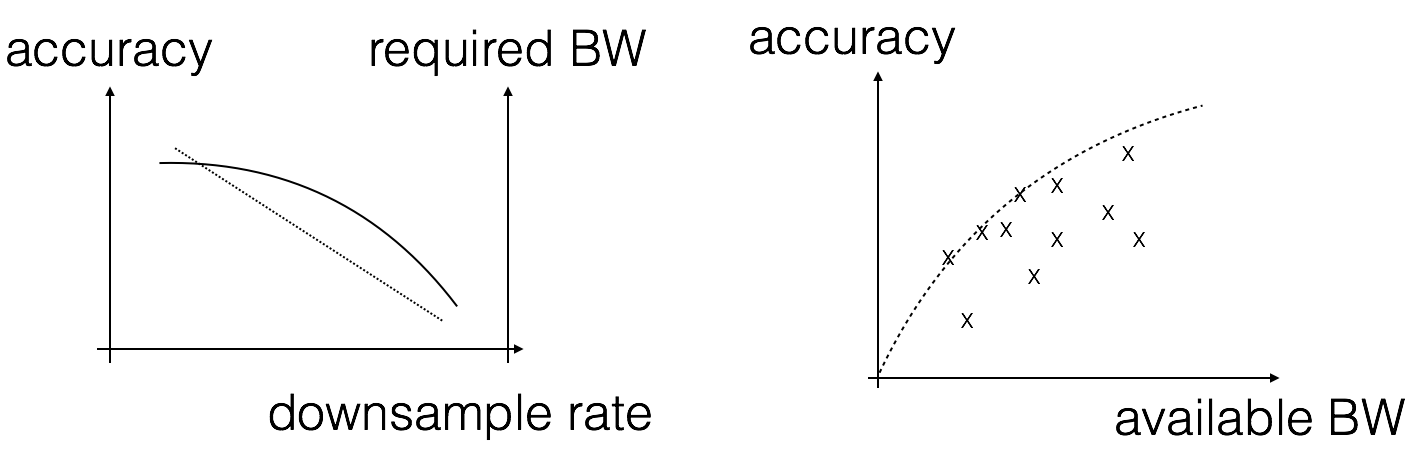
\includegraphics[width=.95\linewidth]{figures/tradeoff-placeholder.png}
  \caption{Application Profiles}
  \label{fig:eval-profile}
\end{figure}

\begin{figure}
  \centering
  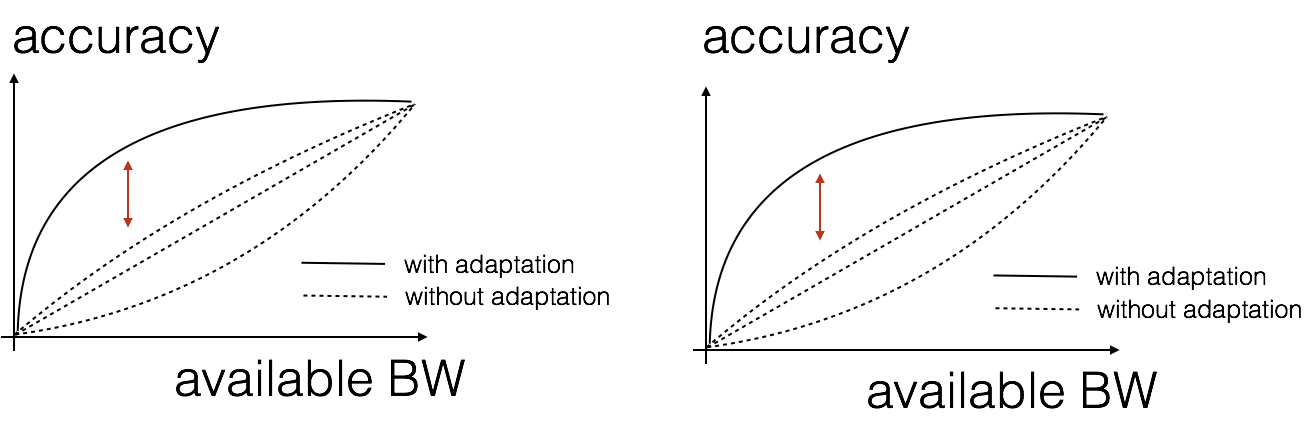
\includegraphics[width=.95\linewidth]{figures/degrade-placeholder.png}
  \caption{Effect on degraded performance: \texttt{ApplicationAware} in
    comparison to \texttt{RandomDrop}, \texttt{BurstDrop},
    \texttt{Backlogged}. left: application 1; right: application 2}
  \label{fig:degrade}
\end{figure}

\begin{figure}
  \centering
  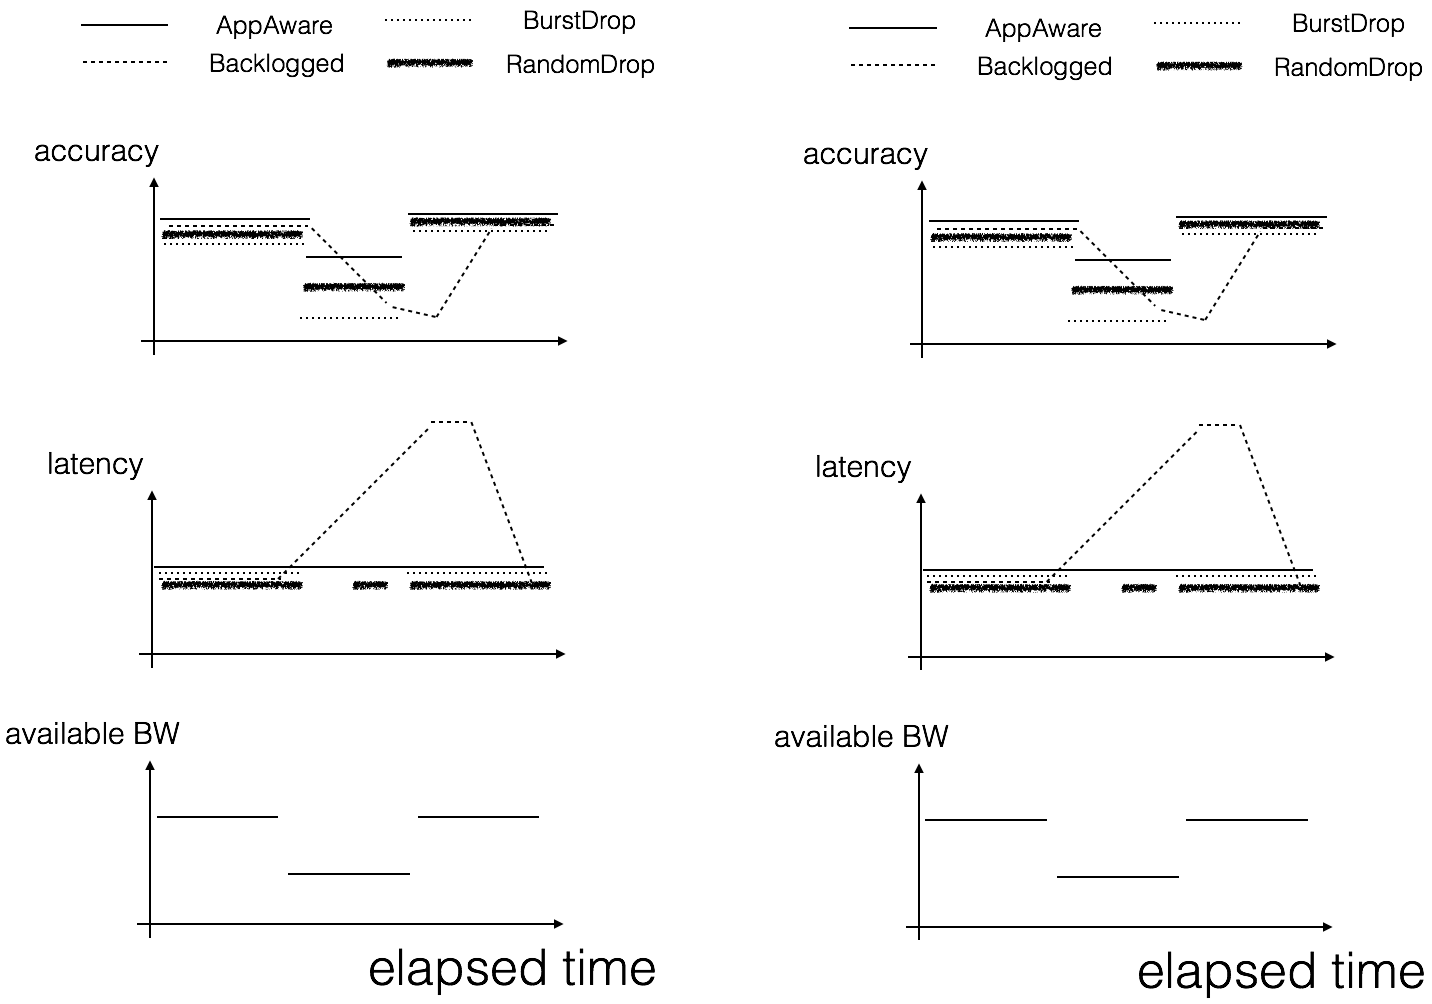
\includegraphics[width=.95\linewidth]{figures/degrade-placeholder-2.png}
  \caption{Effect on degraded performance in a time-series view:
    \texttt{ApplicationAware} in comparison to \texttt{RandomDrop},
    \texttt{BurstDrop}, \texttt{Backlogged}. left: application 1; right:
    application 2}
  \label{fig:degrade-ts}
\end{figure}

\subsection{Overhead}
\label{sec:overhead}

In this section, we evaluate the overhead of the base system with
microbenchmarks.

%%% Local Variables:
%%% mode: latex
%%% TeX-master: "sigcomm2017"
%%% End:
